\documentclass[crop,tikz]{standalone}
\usepackage{tikz}

\begin{document}
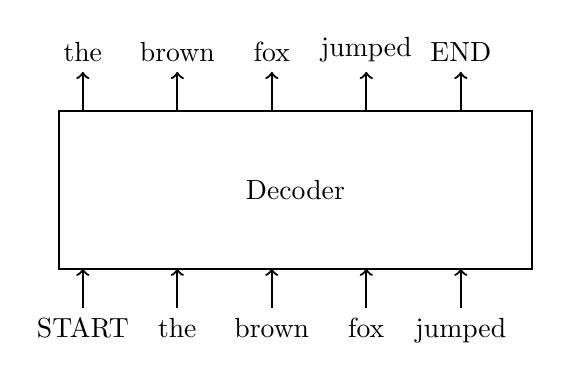
\begin{tikzpicture}
% Rectangle
\draw[thick] (0,0) rectangle (6,2);
\node at (3,1) {Decoder};
% Arrows below
\foreach \i/\j in {0/START,1/the,2/brown,3/fox,4/jumped}
    \draw[<-,thick] (\i*1.2+0.3,0) -- (\i*1.2+0.3, -0.5) node[below] {\j};
% Arrows above
\foreach \i/\j in {0/the,1/brown,2/fox,3/jumped,4/END}
    \draw[->,thick] (\i*1.2+0.3,2) -- (\i*1.2+0.3, 2.5) node[above] {\j};
\end{tikzpicture}
\end{document}

